\chapter{Introduction}
\section{Neutrinos Oscillation}
The Standard Model of elementary particle interactions provides an accurate description of strong, weak, and electromagnetic interactions, but it treats these interactions as distinct and unrelated. Within this framework, neutrinos are assumed to be massless, but this assumption has been called into question by physicists. Neutrino oscillations, which occur when neutrinos change from one flavor to another, are a potential indication of neutrino mass.\\
The term "neutrino oscillations" refers to this phenomena and it involve the conversion of a neutrino of a particular flavor to another as it propagates through space.

Each known flavor eigenstate, $(\nu_e,\nu_{\mu},\nu_{\tau})$, linked to three respective charged leptons $(e,\mu,\tau)$  via the charged current interactions can be considered a complex combination of neutrino mass eigenstates as follow:

\begin{equation*}
	\left(\begin{array}{l}
		v_e \\
		v_\mu \\
		v_\tau
	\end{array}\right)=U_{\mathrm{PMNS}}\left(\begin{array}{l}
		v_1 \\
		v_2 \\
		v_3
	\end{array}\right)
\end{equation*}
in wich $\nu_i$ are the three mass eigensates, that have 3 masses  $m_i$  $(i = 1,2,3)$, which are non-degenerate, with $m_i \neq m_j$ for $i \neq j$.\\

The matrix $U_{\mathrm{PMNS}}$, called Pontecorvo-Maki-Nakagawa-Sakata (PMNS) matrix, is composed of three rotation matrices, $R_{23}$, $R_{13}$, and $R_{12}$, each corresponding to a different mixing angle, $\theta_{23}$, $\theta_{13}$, and $\theta_{12}$, respectively and a parameter $\delta_{CP}$ called the Dirac CP-violating phase. For this case, the Majorana $C P$ phases are $eta i(i=1,2)$, which are only physically possible if neutrinos are Majorana-type particles and do not participate in neutrino oscillations. Therefore, $U$ can be expressed as:

\begin{equation*} 
	\begin{split}
			U_{\text {PMNS }}&=\\
		=&\left(\begin{array}{ccc}
			1 & 0 & 0 \\
			0 & c_{23} & s_{23} \\
			0 & -s_{23} & c_{23}
		\end{array}\right) \left(\begin{array}{ccc}
			c_{13} & 0 & s_{13} \mathrm{e}^{-\mathrm{i} \delta_{C P}} \\
			0 & 1 & 0 \\
			-s_{13} \mathrm{e}^{\mathrm{i} \delta_{C P}} & 0 & c_{13}
		\end{array}\right) 
		\left(\begin{array}{ccc}
			c_{12} & s_{12} & 0 \\
			-s_{12} & c_{12} & 0 \\
			0 & 0 & 1
		\end{array}\right)\left(\begin{array}{ccc}
			\mathrm{e}^{\mathrm{i} \eta_1} & 0 & 0 \\
			0 & \mathrm{e}^{\mathrm{i} \eta_2} & 0 \\
			0 & 0 & 1
		\end{array}\right)
	\end{split}
\end{equation*}

The theoretical framework for neutrino oscillations involves the calculation of the oscillation probability as a function of the distance traveled by the neutrino, the neutrino mixing matrix, and the difference in squared masses between the three neutrino mass states, $\Delta m_{ij}^2$. Specifically,two nuclear power reactors 53 $\unit{\kilo\meter}$ away from the detector, which mostly produce anti-electron neutrinos $\bar{\nu}_e$ with energy below 10 MeV, are the principal sources of neutrinos for the JUNO experiment. So, it is necessary for the JUNO experiment to calculate the survival probability $P\left(\bar{\nu}_e \rightarrow \bar{\nu}_e\right)$ of electron antineutrinos.

\begin{equation*}
	P\left(\bar{\nu}_e \rightarrow \bar{\nu}_e\right)=1-\sin ^2 2 \theta_{12} c_{13}^4 \sin ^2\left(\frac{\Delta m_{21}^2 L}{4 \mathcal{E}}\right)-\sin ^2 2 \theta_{13}\left[c_{12}^2 \sin ^2\left(\frac{\Delta m_{31}^2 L}{4 \mathcal{E}}\right)+s_{12}^2 \sin ^2\left(\frac{\Delta m_{32}^2 L}{4 \mathcal{E}}\right)\right]
\end{equation*}

where $s_{i j} \equiv \sin \theta_{i j}, c_{i j} \equiv \cos \theta_{i j}, \mathcal{E}$ is the neutrino energy, $L$ the travelled distance and $\Delta m_{i j}^2 \equiv m_i^2-m_j^2$. \\
Past experiments have already given estimates for  $\Delta m_{21}^2,\left|\Delta m_{31}^2\right|$ and the  3 mixing angles. 


\begin{figure}[h]
	\centering
	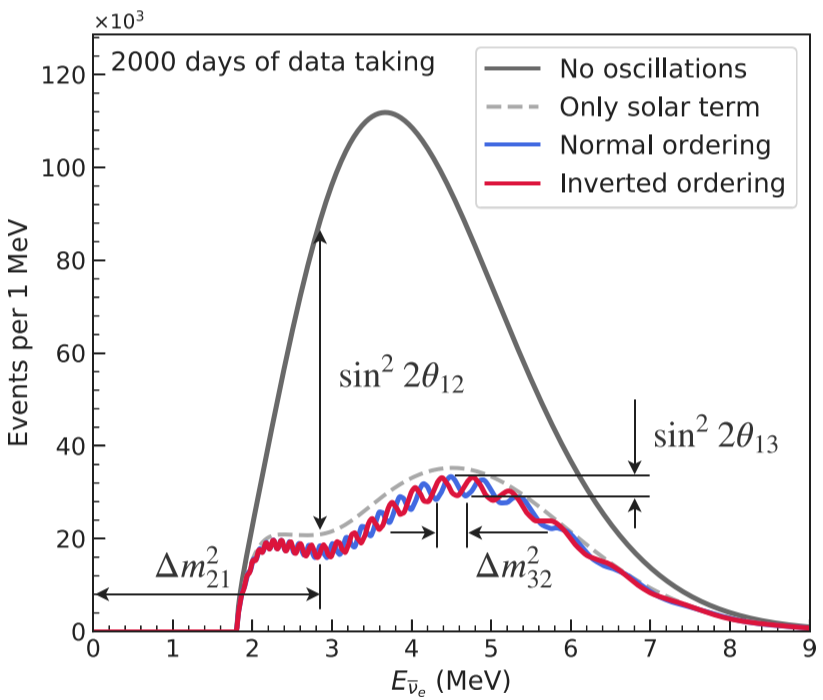
\includegraphics[width=0.4\linewidth]{Images/antineutino_to_antineutrino_probability_plot}
	\caption{JUNO's reactor antineutrino energy spectrum is shown with and without the effect of neutrino oscillation. The gray dashed curve includes only the term in the disappearance probability modulated by $sin^2(2\theta_{12})$, while the blue and red curves use the full oscillation probability for normal and inverted mass orderings. Spectral features driven by oscillation parameters are illustrated, highlighting the rich information available in JUNO's high-resolution measurement of the oscillated spectrum.}
	\label{fig:antineutinotoantineutrinoprobabilityplot}
\end{figure}


%TODO: Questo paragrafo da modificare come è scritto, FrMa
The aim of JUNO is then to improve these results, and especially fix the sign of $\Delta m_{31}^2$ by discriminating between two possibilities:\textit{ Normal Ordering} (\textbf{NO}), where $\left|\Delta m_{31}^2\right|=\left|\Delta m_{32}^2\right|+\left|\Delta m_{21}^2\right|$, and if $m_1<m_2<m_3$ we have the so called \textit{ Inverted Ordering} (\textbf{IO}), where $\left|\Delta m_{31}^2\right|=\left|\Delta m_{32}^2\right|-\left|\Delta m_{21}^2\right|$, and $m_3<m_1<m_2$.
In fact, depending on the sign of $\Delta m_{31}^2$, the plot of \ref{fig:antineutinotoantineutrinoprobabilityplot} is minimally different.


\section{The JUNO detector}

The Jiangmen Underground Neutrino Observatory (JUNO) is an experiment that is currently under construction in Southern China. It is a multipurpose experiment that will use a 20 kton liquid scintillator (LS) detector, a water Cherenkov detector in which the detector is submerged, and a plastic scintillator array on the top of them to study neutrinos from a variety of natural sources as well as from nuclear reactors.

A schematic illustrating the location of both JUNO and TAO is shown in Fig. \ref{fig:junoschemeexperiment}.

\begin{figure}[h]
	\centering
	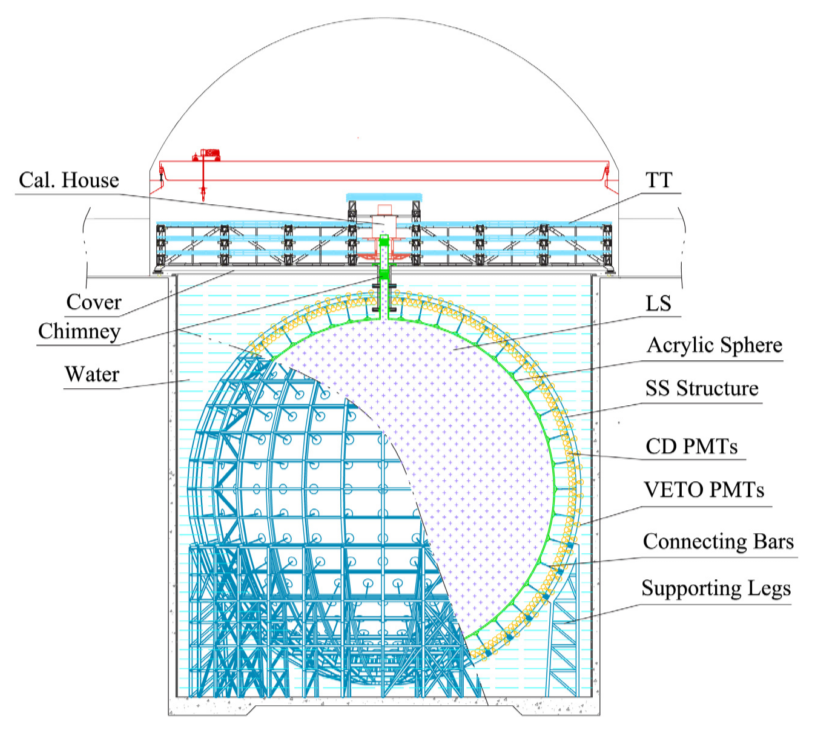
\includegraphics[width=0.7\linewidth]{Images/juno_scheme_experiment}
	\caption[JUNO scheme experiment]{Schematic view of the JUNO experiment}
	\label{fig:junoschemeexperiment}
\end{figure}

%TAO
JUNO is expected to detect a large number of antineutrinos from nuclear reactors, with most of them originating from the Taishan and Yangjiang nuclear power plants (NPPs). These two plants are located at a baseline of about 52.5 km from the JUNO detector, which was optimized for the best sensitivity to the neutrino mass ordering, and have a combined nominal thermal power of 26.6 $GW_{th}$. However, in order to precisely measure the unoscillated reactor antineutrino spectrum shape, a dedicated small satellite detector called TAO will be placed at about 30 m from one of the Taishan reactors. TAO will serve as a data-driven input to constrain the spectra of the other cores.\\

%LIQUID SCINTILLATOR
To achieve its scientific goals, JUNO employs a large liquid scintillator detector with a fiducial mass of 20 kton. The detector is located in a cylindrical cavity excavated under a hill in Jiangmen City, Guangdong Province, China, at a depth of 700 m.w.e. to reduce background radiation from cosmic rays. The scintillator is doped with a small amount of gadolinium to enhance its sensitivity to antineutrinos via the inverse beta decay (IBD) process. The liquid scintillator used in JUNO is a combination of LAB (linear alkyl benzene) and PPO (2,5-diphenyloxazole) doped with a small amount of bis-MSB (1,4-bis(2-methylstyryl) benzene). When a neutrino interacts with the scintillator, it can produce charged particles such as electrons, protons, and alpha particles that travel through the scintillator and excite the scintillation molecules. This excitation results in the emission of photons with a wavelength of around 430 nm. These photons are detected by 20,000 20-inch photomultiplier tubes (PMTs) distributed in a 3-dimensional arrangement inside the detector.\\


The PMTs detect the light and convert it into an electrical signal. The signals from all the PMTs are then combined to reconstruct the position and energy of the original neutrino interaction. This technique allows JUNO to measure the energy of the incoming neutrino to high precision, which is crucial for studying neutrino oscillation.

Moreover, the scintillator's composition and the detector's design are optimized to reduce background noise from other sources of radiation, such as cosmic rays and natural radioactivity. By carefully controlling these backgrounds, JUNO aims to achieve a signal-to-background ratio of better than 1:10,000, which is essential for observing the subtle effects of neutrino oscillation.


In JUNO's location, the energy spectrum will be distorted by two types of oscillations. The first is a slow (low frequency) oscillation driven by $\Delta m_{21}^2$ and modulated by $\sin ^2 \theta_{12}$, while the second is a fast (high frequency) oscillation driven by $\Delta m_{31}^2$ and modulated by $\sin ^2 \theta_{13}$. Fitting the data spectrum against the predicted spectrum distorted by standard neutrino oscillations enables measuring the oscillation parameters.\\

In addition to studying reactor antineutrinos, JUNO will also investigate neutrinos from natural sources such as the Sun, supernovae, and atmospheric neutrinos.

\section{JUNO signal and background}
\subsection{Signal}


\subsection{Background}
Several different types of backgrounds signal are produced in the detector. For analysis we deeply analysed only the three most important contributes:
\paragraph{Muons}

\paragraph{Accidental Coincidence}


\paragraph{Multiple antineutrino sources} 